\chapter{黑洞、吸积盘与 photon ring}
\label{chap:e19}

\begin{chapteropening}
黑洞没有可以反光的固体表面，我们从来没有"看见"过黑洞本身。我们看见的，是它周围被烧得发亮的气体，以及被它极端引力反复弯折的光路。想象一支火把绕着一口深不见底的井转圈：火焰本身是吸积盘的辐射，而井口那一圈幽暗轮廓，是光线在坠入之前最后绕行留下的边界——这就是黑洞阴影（black hole shadow）与它外缘那道细亮的 photon ring（光子环）。本章要把这幅画面讲清楚：吸积盘为什么会发光、发多亮、颜色怎么排布；强引力透镜如何把远处的光弯成一圈；这圈光在天空上有多大、为什么恰好落在 EHT 甚长基线阵列能分辨的门槛上；photon ring 内部为什么藏着一层层自相似的子环；最后，把前两部分学到的相干与干涉工具（\ref{chap:e08}、\ref{chap:e10}、\ref{chap:e11}）接上来，看看长基线和 \(|V|^2\) 的环状振荡在原理上还能为黑洞边缘补充什么。
\end{chapteropening}

\section{黑洞的尺度怎样定下所有坐标}
\label{sec:e19-scales}

在讨论任何具体现象之前，先要有一把尺子。黑洞问题最省事的地方，是它只有一个真正的主导参数：质量 \(M\)。一旦给定 \(M\)，长度、时间、天空角尺度就全部被锁定，剩下的物理都可以用无量纲的比值来谈。我们把这三把标尺写下来：
\begin{equation}
  r_g=\frac{GM}{c^2},\qquad
  t_g=\frac{GM}{c^3}=\frac{r_g}{c},\qquad
  \theta_g=\frac{r_g}{D}.
  \label{eq:e19-scales}
\end{equation}
\begin{formulaexplain}
\(r_g\) 是引力半径（长度），\(t_g\) 是光走过一个 \(r_g\) 的时间，\(\theta_g\) 是把 \(r_g\) 放到距离 \(D\) 处看到的角尺度。三者都正比于质量。
\end{formulaexplain}
这里 \(r_g\) 称为引力半径（gravitational radius），量纲是长度，常用 km 或 cm；它大约是史瓦西半径的一半（\(r_s=2r_g\)）。\(t_g\) 是把 \(r_g\) 除以光速得到的光行时，量纲是时间；它是黑洞附近一切动力学过程的"最快节拍"。\(D\) 是我们到黑洞的距离，\(\theta_g=r_g/D\) 是把这把长度尺子投影到天球上得到的角尺度，量纲是弧度，但天文上更常用微角秒（\(\mu{\rm as}\)，即 \(10^{-6}\) 角秒）。

先把最有用的数字算出来。在 CGS 单位下 \(G=6.674\times10^{-8}\,{\rm cm^3\,g^{-1}\,s^{-2}}\)，太阳质量 \(M_\odot=1.989\times10^{33}\,{\rm g}\)，于是 \(GM_\odot=1.327\times10^{26}\,{\rm cm^3\,s^{-2}}\)。代入 \(r_g\)：
\[
  r_g(M_\odot)=\frac{1.327\times10^{26}}{(2.998\times10^{10})^2}\,{\rm cm}
  =1.477\times10^{5}\,{\rm cm}=1.477\,{\rm km},
\]
再除以光速得到光行时：
\[
  t_g(M_\odot)=\frac{r_g}{c}=\frac{1.477\times10^{5}\,{\rm cm}}{2.998\times10^{10}\,{\rm cm\,s^{-1}}}
  =4.93\times10^{-6}\,{\rm s}=4.93\,\mu{\rm s}.
\]
把这两个"每太阳质量"的基准写成标度式，方便随手换算：
\begin{equation}
  r_g=1.477\,{\rm km}\left(\frac{M}{M_\odot}\right),\qquad
  t_g=4.93\,\mu{\rm s}\left(\frac{M}{M_\odot}\right).
  \label{eq:e19-scalenum}
\end{equation}
\begin{formulaexplain}
把质量以太阳质量为单位代进去，就直接读出引力半径（公里）和光行时（微秒）。同一套无量纲吸积过程，因质量不同会被拉到完全不同的时间尺度。
\end{formulaexplain}

这一步的物理意义值得停下来体会。取两个真实目标。银河系中心的 Sgr~A* 质量约 \(M\simeq4\times10^6\,M_\odot\)，所以 \(t_g\simeq4.93\,\mu{\rm s}\times4\times10^6\simeq20\,{\rm s}\)：靠近最内稳定圆轨道（ISCO）的物质，其结构变化只需几分钟就能显现。相比之下 M87* 的质量 \(M=(6.5\pm0.7)\times10^9\,M_\odot\)，\(t_g\simeq4.93\,\mu{\rm s}\times6.5\times10^9\simeq3.2\times10^4\,{\rm s}\simeq9\,{\rm h}\)：同样的无量纲过程会被拉长到小时甚至天的量级。于是 Sgr~A* 会在一次 VLBI 观测夜里"抖动"，而 M87* 近乎静止——这不是两种物理，而是同一种物理套在相差约 \(10^3\) 的质量上 \citep{2019ApJ...875L...1E,2019ApJ...875L...6E,2022ApJ...930L..12E}。

角尺度更有戏剧性。取常用距离，Sgr~A* 约 \(D\simeq8\,{\rm kpc}\)，M87* 约 \(D\simeq16.8\,{\rm Mpc}\)。这里要小心：\(\theta_g=r_g/D\) 只有在分子分母同单位时才是弧度，所以先把距离化成 cm。用 \(1\,{\rm kpc}=3.086\times10^{21}\,{\rm cm}\)，Sgr~A* 的 \(D=8\,{\rm kpc}=2.47\times10^{22}\,{\rm cm}\)，而它的引力半径 \(r_g=1.477\,{\rm km}\times4\times10^6=5.91\times10^{11}\,{\rm cm}\)。先算出以弧度计的角尺度，再乘 \(1\,{\rm rad}=2.063\times10^{11}\,\mu{\rm as}\) 换成微角秒：
\[
  \theta_g^{\rm SgrA*}=\frac{r_g}{D}
  =\frac{5.91\times10^{11}\,{\rm cm}}{2.47\times10^{22}\,{\rm cm}}
  =2.39\times10^{-11}\,{\rm rad}
  \times 2.063\times10^{11}\,\frac{\mu{\rm as}}{\rm rad}
  \approx 4.9\,\mu{\rm as}.
\]
M87* 同法：\(r_g=1.477\,{\rm km}\times6.5\times10^9=9.6\times10^{14}\,{\rm cm}\)，\(D=16.8\,{\rm Mpc}=5.18\times10^{25}\,{\rm cm}\)，得 \(\theta_g^{\rm M87*}=1.85\times10^{-11}\,{\rm rad}\approx3.8\,\mu{\rm as}\)。质量相差 \(10^3\)、距离也相差约 \(10^3\)，两个 \(\theta_g\) 便都落在几微角秒。把 \(\theta_g\) 乘上下一节要讲的阴影系数 \(\kappa\simeq10.4\)，就得到几十微角秒的阴影——这正是 EHT 的观测门槛。图~\ref{fig:e19-scales} 把这层"质量线性控制一切"的关系画了出来。

\begin{figure}[tbp]
\centering
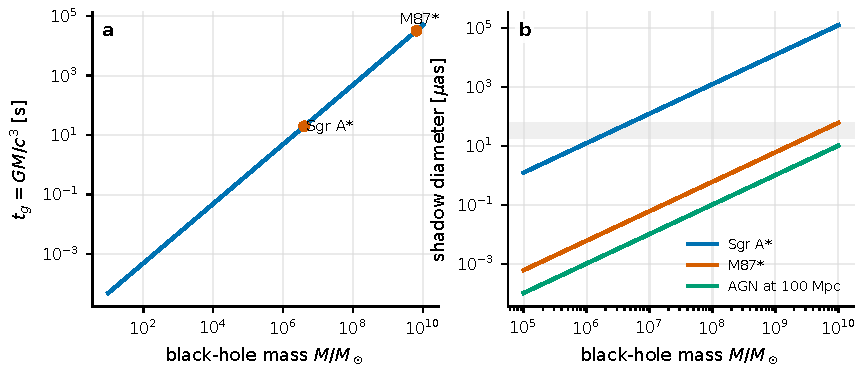
\includegraphics[width=0.94\linewidth]{figures/generated/chapter_12/ch12_black_hole_scales.pdf}
\caption{黑洞的时间尺度和角尺度都由质量线性控制。Sgr~A* 和 M87* 的质量相差约 \(10^3\)，但距离也相差约 \(10^3\)，所以二者的阴影角直径都在几十微角秒；时间尺度却完全不同：Sgr~A* 可以在一次 VLBI 扫描内改变，M87* 的结构更接近静态。}
\label{fig:e19-scales}
\end{figure}

有了尺子，就可以把黑洞观测的"事件表坐标"写全。前几章我们把一次光子探测记成到达时间和频率；到了黑洞成像，坐标要扩展为
\[
  (t_i,\ \nu_i,\ \bm{b}_i,\ \eta_i,\ w_i),
\]
其中 \(t_i\) 是到达时间，\(\nu_i\) 是频率或能道，\(\bm{b}_i\) 是投影基线（决定测到哪个空间频率），\(\eta_i\) 是偏振通道，\(w_i\) 是权重。EHT 的复可见度、GRAVITY 的差分相位、光学监测的光变，都可以看成这张事件表的不同投影。关键在于：投影之前尽量保留时间和偏振，才能把吸积流变化、喷流扰动和强引力多路径分开估计。这条思路和 \ref{chap:e11} 里"从可见度到成像"是同一套语言，只是现在测量对象换成了强引力弯折过的光。

\section{吸积盘怎样产生连续谱和随机光变}
\label{sec:e19-disk}

黑洞不发光，发光的是落向它的气体。气体带着角动量，无法直接掉进去，只能盘旋着一圈圈向内、彼此摩擦、把引力势能磨成热，最后辐射出去——这就是吸积盘（accretion disk）。标准薄盘模型给出单位面积的辐射通量：
\begin{equation}
  F(R)=\frac{3GM\dot M}{8\pi R^3}
  \left[1-\left(\frac{R_{\rm in}}{R}\right)^{1/2}\right],
  \label{eq:e19-flux}
\end{equation}
\begin{formulaexplain}
\(F(R)\) 是盘上半径 \(R\) 处单位面积向外辐射的功率，\(\dot M\) 是吸积率，\(R_{\rm in}\) 是内边界。方括号让通量在内边界处归零。
\end{formulaexplain}
逐个符号看：\(R\) 是盘半径（cm），\(\dot M\) 是吸积率（\({\rm g\,s^{-1}}\)），\(R_{\rm in}\) 是盘的内边界，通常取几倍 \(r_g\)（对无自旋黑洞 ISCO 在 \(6r_g\)）。方括号 \([\,1-(R_{\rm in}/R)^{1/2}\,]\) 保证物质在内边界处不再有净力矩、通量趋零；一旦 \(R\gg R_{\rm in}\)，方括号趋近 1，主导行为就是 \(F\propto R^{-3}\)。

若盘在局部近似黑体，把通量换成温度：
\begin{equation}
  T(R)=\left[\frac{F(R)}{\sigma_{\rm SB}}\right]^{1/4},
  \label{eq:e19-temp}
\end{equation}
\begin{formulaexplain}
\(T(R)\) 是盘在半径 \(R\) 的局部有效温度，\(\sigma_{\rm SB}\) 是 Stefan--Boltzmann 常数。薄盘光谱的颜色，是不同半径黑体温度叠加出来的。
\end{formulaexplain}
在远离内边界处 \(F\propto R^{-3}\)，代入并注意四次方根：
\[
  T(R)\propto \big(R^{-3}\big)^{1/4}=R^{-3/4}
  \quad\Longrightarrow\quad
  T(R)\propto (M\dot M)^{1/4}\,R^{-3/4}.
\]
这就是薄盘最著名的温度律：越往里越热，颜色越蓝。现在问一个观测者会问的问题——某个波长 \(\lambda\) 主要来自哪个半径？黑体在波长 \(\lambda\) 处最亮时满足 Wien 关系 \(k_{\rm B}T\sim hc/\lambda\)，也就是 \(T\propto1/\lambda\)。把这个条件塞进温度律：
\[
  \frac{1}{\lambda}\propto (M\dot M)^{1/4}R_\lambda^{-3/4}
  \;\Longrightarrow\;
  R_\lambda^{3/4}\propto (M\dot M)^{1/4}\lambda
  \;\Longrightarrow\;
  R_\lambda\propto (M\dot M)^{1/3}\lambda^{4/3}.
\]
写成标度式：
\begin{equation}
  R_\lambda \propto (M\dot M)^{1/3}\,\lambda^{4/3}.
  \label{eq:e19-Rlambda}
\end{equation}
\begin{formulaexplain}
\(R_\lambda\) 是波长 \(\lambda\) 附近主要发光的盘半径。波长越长来自越外层；质量和吸积率越大，同一颜色的发光环也越大。
\end{formulaexplain}
这条 \(R_\lambda\propto\lambda^{4/3}\) 是可以被观测检验的"指纹"。对 \(M\sim10^8\,M_\odot\)、爱丁顿比 \(L/L_{\rm Edd}\sim0.1\) 的类星体，光学到近紫外连续谱大致来自 \(0.1\)–\(10\) 光日（light-day）量级的半径。有意思的是，微透镜和多波段延迟测量经常给出比最简薄盘更大的光学盘，这正是非均匀盘（inhomogeneous disk）和再处理（reprocessing）模型被反复讨论的原因 \citep{1973A&A....24..337S,2006ApJ...642...87P,2011ApJ...727L..24D}。图~\ref{fig:e19-disk} 左侧的橙色区域就示意了这种"实测光学盘偏大"的情形。

\begin{figure}[tbp]
\centering
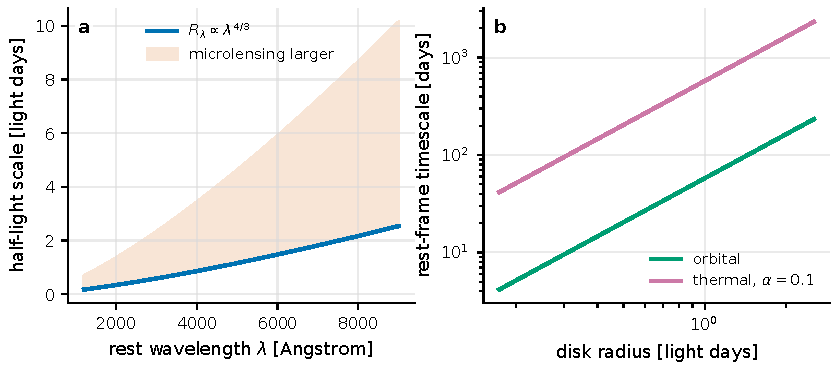
\includegraphics[width=0.94\linewidth]{figures/generated/chapter_12/ch12_accretion_disk_radii.pdf}
\caption{薄盘标度给出 \(R_\lambda\propto\lambda^{4/3}\)。左图橙色区域表示微透镜和部分连续谱延迟常暗示的更大光学发光面积；右图比较同一半径上的轨道时间和热时间，若 \(\alpha\simeq0.1\)，热时间约为轨道时间的十倍。}
\label{fig:e19-disk}
\end{figure}

发光是一幅静态图，但吸积盘还在不停"闪烁"。要理解光变的时间尺度，先估计盘上一个半径处的两把时钟：
\begin{equation}
  t_{\rm orb}=2\pi\left(\frac{R^3}{GM}\right)^{1/2},\qquad
  t_{\rm th}\simeq\frac{t_{\rm orb}}{\alpha}.
  \label{eq:e19-times}
\end{equation}
\begin{formulaexplain}
\(t_{\rm orb}\) 是开普勒轨道周期，\(t_{\rm th}\) 是热时间（局部储能被辐射改写所需的时间），\(\alpha\) 是粘滞参数。扰动落在哪把时钟上，决定光变能多快响应。
\end{formulaexplain}
\(t_{\rm orb}\) 就是把开普勒第三定律 \(\Omega^2=GM/R^3\) 取周期 \(2\pi/\Omega\) 得到的轨道时间；\(t_{\rm th}\) 是热时间，即局部储热被辐射重新分配所需的时间。\(\alpha\) 是 Shakura--Sunyaev 粘滞参数（无量纲），常取 \(0.01\)–\(0.3\)。因为 \(\alpha<1\)，热时间总比轨道时间长，图~\ref{fig:e19-disk} 右侧取 \(\alpha\simeq0.1\) 时二者相差约十倍。对 AGN 光学盘，\(t_{\rm orb}\) 可以是几十天到几年，\(t_{\rm th}\) 更长——这就是为什么类星体的光学光变以"月到年"为节拍。

大样本光学光变常用阻尼随机游走（damped random walk, DRW）来描述，它的自协方差和功率谱是一对：
\begin{equation}
  C(\tau)=\sigma^2\exp\!\left(-\frac{|\tau|}{\tau_d}\right),
  \qquad
  P(f)\propto\frac{1}{1+(2\pi f\tau_d)^2}.
  \label{eq:e19-drw}
\end{equation}
\begin{formulaexplain}
\(C(\tau)\) 是光变的自协方差，\(\tau_d\) 是阻尼（记忆）时间，\(P(f)\) 是功率谱。这个模型把随机光变写成一个"会慢慢忘掉自己"的相关过程。
\end{formulaexplain}
先点名符号：\(\sigma^2\) 是光变的方差（长时间尺度上亮度起伏振幅的平方），因此 \(\sigma\) 与被测的亮度（或流量）同量纲，量纲就是流量/星等的量纲；\(\tau\) 是时间延迟，\(f\) 是频率。这里两式互为傅里叶变换：指数型自协方差的谱是洛伦兹型（\ref{chap:e02} 里我们正是用这一对关系把相关时间和带宽联系起来的）。物理图像很直白：\(\tau_d\) 是盘"记得自己上一刻多亮"的时间；比 \(\tau_d\) 短的时标上光变高度相关，比它长就渐渐失忆，功率谱在 \(f\gtrsim1/2\pi\tau_d\) 处转入 \(f^{-2}\) 衰减。观测上 \(\tau_d\) 与黑洞质量相关，超大质量黑洞常为数十到数百天（静止系）\citep{1993ApJ...406..420M,2021Sci...373..789B,2016Natur.534...75M}。图~\ref{fig:e19-var} 对比了短、长两种 \(\tau_d\) 的记忆行为。

\begin{figure}[tbp]
\centering
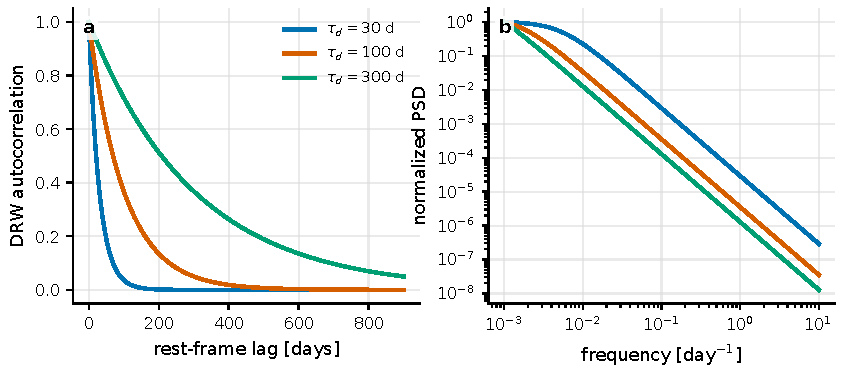
\includegraphics[width=0.94\linewidth]{figures/generated/chapter_12/ch12_variability_autocorrelation.pdf}
\caption{阻尼随机游走把随机光变写成一个相关时间。短 \(\tau_d\) 的光变很快失去记忆，功率谱较早转入 \(f^{-2}\) 衰减；长 \(\tau_d\) 的盘在更长时间上保持相关，低频平台延伸得更远。}
\label{fig:e19-var}
\end{figure}

这里要给对光子统计感兴趣的读者一句诚实的提醒。前几章的 \(g^{(2)}\) bunching（\ref{chap:e08}）是单模热光的量子指纹；但一个 \(10^8\,M_\odot\) 的 AGN 光学连续谱来自海量彼此独立的湍流小区和多个热时间的叠加，属于极端多模。多模会把每一模的 bunching 平均掉，测到的 \(g^{(2)}\) 几乎压到 1。所以吸积盘上更现实的可测量，不是原始 bunching，而是在相位或颜色条件下的"过量相关"——例如比较 flare 前后 \(g^{(2)}(\tau)\) 宽度的变化，或把偏振通道分开来读湍流胞元的寿命。平均亮度主要给出光子率和归一化；能不能真正测到相关，还受相干时间、采样窗口和经典涨落可否建模的联合约束。

\section{强引力透镜与 photon ring 的几何起源}
\label{sec:e19-geometry}

现在走到本章的核心画面：那圈亮环是怎么来的。关键在于，黑洞附近的光不走直线。想象你站在很远处，向黑洞方向平行射出许多光线，每条光线用它的碰撞参数（impact parameter）\(b\) 标记——\(b\) 就是"如果没有引力，这条光线会从黑洞旁多远处擦过"。引力会把光线往里掰：
\begin{itemize}
\item \(b\) 很大时，光线只被轻微偏折，径直飞过；
\item \(b\) 逐渐减小，偏折越来越狠，光线开始绕黑洞转小半圈、一圈、几圈；
\item 存在一个临界值 \(b_c\)：恰好等于它时，光线会无限逼近某个圆轨道盘旋不去；小于它，光线一头栽进黑洞，再也出不来。
\end{itemize}
那个让光"能绕圈"的圆轨道，叫光子球（photon sphere）。对无自旋（史瓦西）黑洞，光子球半径和临界碰撞参数是标准的广义相对论结果：
\begin{equation}
  r_{\rm ph}=3\,\frac{GM}{c^2}=3\,r_g,\qquad
  b_c=3\sqrt{3}\,\frac{GM}{c^2}=3\sqrt{3}\,r_g\approx5.196\,r_g.
  \label{eq:e19-photonsphere}
\end{equation}
\begin{formulaexplain}
\(r_{\rm ph}\) 是光子能做圆周运动的半径，\(b_c\) 是能逃逸与被吞没之间的临界碰撞参数。它们只依赖 \(r_g\)，也就是只依赖质量。
\end{formulaexplain}
这两个数怎么理解？\(r_{\rm ph}=3r_g\) 说明光子球坐落在史瓦西半径（\(2r_g\)）之外一点，是"光还能勉强绕圈但极不稳定"的地方；任何微小扰动都会让绕行的光要么向内坠落、要么向外逃逸。\(b_c=3\sqrt3\,r_g\) 则是天球上的分界线：来自背景、碰撞参数 \(b<b_c\) 的光都进了黑洞，于是我们看到一块暗斑；\(b\) 稍大于 \(b_c\) 的光会绕行若干圈后逃出，叠在暗斑外缘，堆成一道细亮的环。这道环就是 photon ring。

暗斑的大小是可以直接算的。观测者看到的阴影半径正是临界碰撞参数投影到天空的角度，阴影角直径为
\begin{equation}
  d_{\rm sh}=\frac{2b_c}{D}=6\sqrt{3}\,\frac{r_g}{D}=6\sqrt{3}\,\theta_g\simeq10.4\,\theta_g,
  \label{eq:e19-shadow}
\end{equation}
\begin{formulaexplain}
\(d_{\rm sh}\) 是黑洞阴影的角直径，等于 \(2b_c\) 除以距离。系数 \(6\sqrt3\approx10.4\) 是纯几何常数，把引力半径角尺度放大约十倍。
\end{formulaexplain}
这一步把上一节埋下的系数 \(\kappa\simeq10.4\) 兑现了：它不是拟合出来的经验数，而是 \(6\sqrt3\) 这个几何常数。对旋转（Kerr）黑洞，自旋和倾角会让阴影略微不圆、系数在百分之几到十来个百分点内浮动，但量级不变，所以我们仍可放心地用 \(d_{\rm sh}\simeq10.4\,\theta_g\) 做估计。

代入上一节的角尺度就得到可观测的环。M87* 的 \(\theta_g\simeq3.8\,\mu{\rm as}\)，预言 \(d_{\rm sh}\simeq10.4\times3.8\simeq40\,\mu{\rm as}\)；EHT 在 \(1.3\,{\rm mm}\) 实测到的非对称环直径为 \(42\pm3\,\mu{\rm as}\)，环中心亮度被压低超过十倍——正是阴影。Sgr~A* 的 \(\theta_g\simeq4.9\,\mu{\rm as}\)，预言 \(d_{\rm sh}\simeq51\,\mu{\rm as}\)，实测厚环直径 \(51.8\pm2.3\,\mu{\rm as}\)，只是源在观测夜内有明显的分钟到小时级变化 \citep{2019ApJ...875L...4E,2019ApJ...875L...5E,2022ApJ...930L..14E,2022ApJ...930L..15E}。一个纯几何常数 \(6\sqrt3\) 乘上一把由质量定的尺子，就把广义相对论预言压到了两位有效数字，与观测吻合——这是本章最值得记住的画面。

要提醒的是：EHT 看到的亮环并不是数学上无限薄的 photon ring。它是几样东西叠在一起：吸积流本身的直接辐射、绕行半圈左右的"一次透镜像"，以及绕行多圈的高阶 photon subring（光子子环）。吸积流的厚度、光深、湍流和时间平均会把强引力的窄结构涂宽。下一节就来看这层层嵌套的子环。

\section{photon ring 的自相似子环结构}
\label{sec:e19-subring}

photon ring 最迷人的性质，是它内部藏着一套自相似的分层结构。回到几何图像：碰撞参数越接近临界值 \(b_c\)，光在逃逸前绕黑洞的圈数越多。我们按"绕行半圈数"给这些像编号 \(n=0,1,2,\dots\)：\(n=0\) 是几乎不绕的直接像，\(n=1\) 是绕约半圈打到另一侧的一次透镜像，\(n\) 越大绕得越多，也越贴近那条临界曲线。每多绕一圈，对应的亮环就更窄、更暗，并且更逼近同一个极限半径。把第 \(n\) 个子环的角宽度和通量写成标度形式：
\begin{equation}
  w_n\simeq w_0\,e^{-\gamma n},\qquad
  F_n\simeq F_0\,e^{-\beta n}.
  \label{eq:e19-subring}
\end{equation}
\begin{formulaexplain}
\(w_n\) 和 \(F_n\) 是第 \(n\) 个 photon subring 的角宽度和通量。两者都随 \(n\) 指数衰减：子环一层层变窄、变暗，并向临界曲线收拢。
\end{formulaexplain}
这里 \(w_0,F_0\) 是最外层（低阶）结构的宽度和通量标度，\(\gamma\) 与 \(\beta\) 是控制"每绕一圈缩小多少"的衰减指数（无量纲）。指数 \(\gamma\) 由光子球轨道的不稳定性决定——正是那条极不稳定的圆轨道的 Lyapunov 指数，刻画相邻光线在绕行中彼此分离的速率；\(\beta\) 还额外取决于沿途的发射与吸收。物理上，\(w_n\sim e^{-\gamma n}\) 意味着子环以近乎固定的比例逐层变窄，形成一套"环套环"的自相似梯子；而 \(F_n\sim e^{-\beta n}\) 意味着高阶子环虽然位置越来越普适（几乎只由 Kerr 度规决定、与吸积流细节无关），通量却越来越小，越来越难测。

这套自相似结构的意义在于它的普适性：低阶像的形状受吸积流的脏细节污染，但足够高阶的子环几乎只记得时空几何本身。理论对史瓦西黑洞给出很干净的结果——每往高一阶，子环的位置、宽度按大约固定的因子收缩、通量按大约固定的因子变暗，收拢到 \(b_c\) 对应的临界曲线上 \citep{2019PhRvD.100b4018G,2020PhRvD.102l4004G,2020SciA....6.1310J}。Gralla 等强调：在总通量里，高阶 photon ring 往往只占很小一份，直接从图像上分离它们非常困难。这就把问题推向了下一节——如果图像域看不清，能不能换到可见度域去看。

\section{EHT 甚长基线成像与可见度里的环状振荡}
\label{sec:e19-visibility}

要分辨几十微角秒的环，光靠单口径望远镜是没戏的：衍射极限 \(\theta\sim\lambda/D_{\rm tel}\)，在 \(1.3\,{\rm mm}\) 要达到 \(20\,\mu{\rm as}\) 需要口径
\[
  D_{\rm tel}\sim\frac{\lambda}{\theta}
  =\frac{1.3\times10^{-3}\,{\rm m}}{20\,\mu{\rm as}}
  =\frac{1.3\times10^{-3}}{20\times4.848\times10^{-12}\,{\rm rad}}
  \approx1.3\times10^{7}\,{\rm m},
\]
也就是地球直径的量级。这正是甚长基线干涉（VLBI）存在的理由：把分布在全球的望远镜连成一台"地球大小"的合成望远镜。干涉仪不直接给图像，它测的是天空亮度分布的傅里叶分量——复可见度：
\begin{equation}
  V(\bm{u})=\int I(\bm{\theta})\,
  e^{-2\pi i\,\bm{u}\cdot\bm{\theta}}\,d^2\theta,
  \qquad
  \bm{u}=\frac{\bm{B}_\perp}{\lambda}.
  \label{eq:e19-vis}
\end{equation}
\begin{formulaexplain}
\(V(\bm u)\) 是复可见度，\(I(\bm\theta)\) 是天空亮度分布，\(\bm u=\bm B_\perp/\lambda\) 是以波长为单位的投影基线（空间频率）。基线越长，看到的空间频率越高，能分辨的角结构越细。
\end{formulaexplain}
这就是 \ref{chap:e10}、\ref{chap:e11} 里 van~Cittert--Zernike 与"可见度即傅里叶分量"的老朋友，只是现在源是一圈被引力弯出来的光。一个理想化的均匀薄环，它的可见度有一个漂亮的解析形式：
\begin{equation}
  V(u)\simeq J_0(\pi d\,u),
  \label{eq:e19-bessel}
\end{equation}
\begin{formulaexplain}
\(J_0\) 是零阶贝塞尔函数，\(d\) 是环的角直径，\(u\) 是基线长度对应的空间频率。薄环的可见度随基线振荡，并在一系列基线上出现零点。
\end{formulaexplain}
为什么是贝塞尔函数？一个半径固定的细环，把它绕一圈的傅里叶积分做出来，角向积分正好给出 \(J_0\)——这与一个圆孔的衍射会出现贝塞尔型花样是同一类几何。要点是：\(J_0(x)\) 是一条振荡衰减的曲线，在 \(x=2.405,\,5.520,\dots\) 处依次穿零。于是环在可见度上留下的指纹，是一串随基线拉长而出现的\emph{零点与旁瓣}——\(|V|^2\) 呈环状振荡，而不是像一个光滑光斑那样单调下降。

把第一个零点落在哪条基线上算出来，就明白 EHT 为什么"刚好够用"。第一个零点在 \(\pi d\,u=2.405\)，即
\[
  u_{\rm null}=\frac{2.405}{\pi d}=\frac{0.765}{d}.
\]
对 M87* 的 \(d\simeq42\,\mu{\rm as}=2.04\times10^{-10}\,{\rm rad}\)：
\[
  u_{\rm null}=\frac{0.765}{2.04\times10^{-10}}\approx3.8\times10^{9}
  =3.8\,{\rm G}\lambda,
\]
换算成实际基线长度 \(B_\perp=u_{\rm null}\,\lambda=3.8\times10^9\times1.3\times10^{-3}\,{\rm m}\approx4.9\times10^{6}\,{\rm m}\)，约 \(5000\,{\rm km}\)——远小于地球直径。也就是说，地球尺度的 \(1.3\,{\rm mm}\) VLBI 恰好能越过第一个可见度谷，直接在可见度域"摸到"环状结构 \citep{2019ApJ...875L...2E,2019ApJ...875L...3E,2020SciA....6.1310J}。

真实的环不是无限薄的。若环有有限宽度 \(w\)，它相当于把理想 \(J_0\) 乘上一个宽度反比于 \(w\) 的包络：宽的结构在较短基线上就被"抹掉"，窄的结构才能在很长的基线上继续保留振荡。这一点把上一节的自相似子环和可见度域连了起来——见图~\ref{fig:e19-ring}。

\begin{figure}[tbp]
\centering
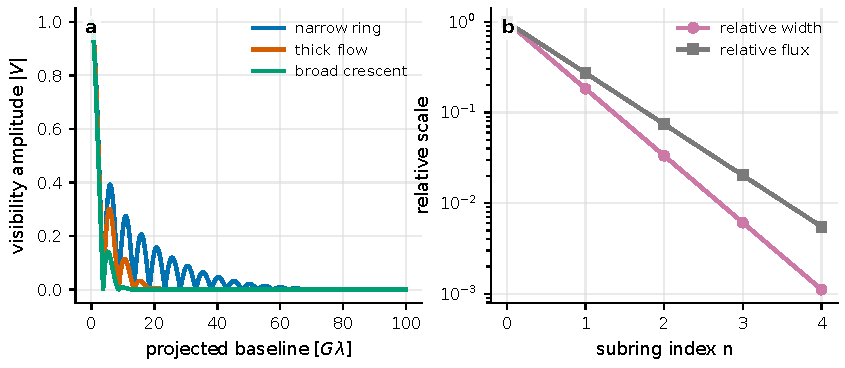
\includegraphics[width=0.94\linewidth]{figures/generated/chapter_12/ch12_photon_ring_visibility.pdf}
\caption{环状结构在长基线可见度中产生振荡。左图比较同样 \(42\,\mu{\rm as}\) 直径下不同厚度的环，窄环在更长基线上仍保留振荡；右图示意 photon subring 的宽度和通量随环绕次数下降，高阶子环通量小，但在足够长的基线上可留下普适的振荡结构。}
\label{fig:e19-ring}
\end{figure}

这就给出了一个漂亮的策略：在图像域里，宽而亮的吸积流盖过了窄而暗的高阶子环；但在可见度域里，随着基线拉长，宽吸积流的贡献先被"解析掉"（其可见度早早衰减到噪声以下），剩下的长基线信号越来越由最窄的 photon subring 主导，露出它那套几乎只由时空几何决定的普适振荡 \citep{2013ApJ...777..170J,2020SciA....6.1310J}。换句话说，够长的基线是一把梳子，能把强引力的普适结构从吸积流的脏背景里梳出来。

\section{干涉与相干方法在原理上还能补充什么}
\label{sec:e19-coherence}

把前两部分的工具接上来，看看它们在原理上能为黑洞边缘结构补充什么。核心有三条。

\textbf{第一，长基线揭示普适子环。} 如上节所述，可见度域的关键资源是基线长度 \(u=B_\perp/\lambda\)。地面 EHT 的基线以地球直径封顶，只够看到第一、第二个可见度谷；要把第 \(n\ge2\) 阶子环那越来越窄、位置越来越普适的振荡挖出来，需要把基线延伸到地球之外（空间 VLBI）或缩短波长。这不是新物理，而是把 \ref{chap:e11} 里"更长基线 = 更高空间频率 = 更细角结构"的原则推到极限：photon ring 的自相似性保证了，只要基线够长，总有一层子环在等着被分辨。

\textbf{第二，\(|V|^2\) 的环状振荡本身就是一种相干测量。} 强度干涉（\ref{chap:e10}）测的正是 \(|V|^2\)（丢掉相位），而环的 \(|V|^2\) 恰恰是一串贝塞尔零点与旁瓣——一种即便没有相位也能识别的"环状指纹"。这为亮、角尺度较大的目标提供了一条不依赖大气相位稳定、可用超长基线的原理性通道：只要能在足够长的基线上测到 \(|V|^2\) 的振荡是否守时、零点落在何处，就能约束环的直径与宽度。代价是强度干涉信号弱、要求极高的光子通量和长积分，对多数黑洞源在近期仍是原理性的而非现成可行的。

\textbf{第三，多路径会在时间结构里留下回声。} 光绕行不同圈数，路径长度不同，到达时间也不同。若第 \(n\) 圈与第 \(n+1\) 圈的平均延迟差接近光子轨道周期 \(T_\gamma\)，那么强度自相关
\begin{equation}
  C(\tau)=\big\langle\delta I(t)\,\delta I(t+\tau)\big\rangle
  \quad\text{可能在}\quad
  \tau\simeq m\,T_\gamma\ (m=1,2,\dots)
  \label{eq:e19-echo}
\end{equation}
\begin{formulaexplain}
\(C(\tau)\) 是强度涨落的自相关，\(T_\gamma\) 是光子绕黑洞一圈的周期，\(m\) 是整数。若多路径贡献可见，自相关会在这些延迟处出现微弱回声峰。
\end{formulaexplain}
附近出现微弱的峰。物理图像是：同一次闪烁的光，一部分直接到达，一部分多绕一圈后晚 \(T_\gamma\) 到达，二者在时间序列里形成"回声"。对 Sgr~A*，\(T_\gamma\) 是分钟量级，正好和吸积流本身的 flare 时标重叠，容易混淆；对 M87*，\(T_\gamma\) 是天量级，源更稳定但观测调度更难。要把这类峰真正解释成强引力多路径，必须先排除喷流激波、盘湍流、散射屏、采样窗口和校准误差——这是一个高门槛的、原理上可行但实践上苛刻的目标。偏振版本还可进一步比较 \(Q,U,V\) 各 Stokes 分量的延迟结构，EHT 对 M87* 和 Sgr~A* 的偏振成像已经展示了这类信息的价值 \citep{2021ApJ...910L..13E,2021PhRvD.104d4049G,2022PhRvD.106d3021C}。

需要给读者一个如实的边界。这些相干手段能补充的是\emph{边缘的角结构与时间结构}，不是黑洞自身的量子辐射。真正属于黑洞本身的量子过程——Hawking 辐射（\ref{chap:e16} 会从辐射机制角度再提）——其温度 \(T_H\propto1/M\) 对恒星质量黑洞已远低于 \(2.725\,{\rm K}\) 的宇宙微波背景，对 Sgr~A*、M87* 更低到 \(10^{-14}\)–\(10^{-17}\,{\rm K}\)，蒸发时标远超宇宙年龄，不在可预见望远镜的灵敏度之内 \citep{1974Natur.248...30H,1975CMaPh..43..199H}。所以对天体质量与超大质量黑洞，近期真正可操作的观测主线仍然是本章讲的这四样：吸积流、偏振、可见度、以及 photon ring 的时间与角结构。

\section{本章要点}
\label{sec:e19-summary}

\begin{itemize}
\item \textbf{一把尺子定全局。} 黑洞的长度、时间、角尺度都正比于质量：\(r_g=1.477\,{\rm km}\,(M/M_\odot)\)，\(t_g=4.93\,\mu{\rm s}\,(M/M_\odot)\)，\(\theta_g=r_g/D\)。Sgr~A* 与 M87* 质量差 \(10^3\)、距离也差 \(10^3\)，故阴影都落在几十微角秒，但时间尺度一为秒、一为小时。
\item \textbf{吸积盘的颜色与闪烁。} 薄盘温度律 \(T\propto R^{-3/4}\) 给出 \(R_\lambda\propto(M\dot M)^{1/3}\lambda^{4/3}\)：波长越长来自越外层。光变以轨道时间和热时间为节拍，可用阻尼随机游走的相关时间 \(\tau_d\) 概括。多模稀释会把原始 bunching 抹平。
\item \textbf{photon ring 的几何起源。} 光子球在 \(r_{\rm ph}=3r_g\)，临界碰撞参数 \(b_c=3\sqrt3\,r_g\)。阴影角直径 \(d_{\rm sh}=6\sqrt3\,\theta_g\simeq10.4\,\theta_g\)——系数是纯几何常数，把 \(\theta_g\) 放大约十倍，预言与 EHT 实测（M87* 约 \(42\,\mu{\rm as}\)、Sgr~A* 约 \(52\,\mu{\rm as}\)）两位有效数字吻合。
\item \textbf{自相似子环。} 高阶子环宽度 \(w_n\sim e^{-\gamma n}\)、通量 \(F_n\sim e^{-\beta n}\) 逐层收窄变暗，向临界曲线收拢；\(\gamma\) 由光子轨道的 Lyapunov 指数决定，越高阶越普适、越难测。
\item \textbf{可见度里的环状指纹。} 薄环可见度 \(V(u)\simeq J_0(\pi d u)\) 在基线上振荡穿零，第一个零点对 M87* 落在约 \(5000\,{\rm km}\) 基线——地球尺度 VLBI 刚好越得过。够长的基线能把宽吸积流解析掉，露出窄子环的普适振荡。
\item \textbf{相干方法能补什么。} 原理上有三条：更长基线揭示更高阶普适子环；\(|V|^2\) 的环状振荡是不依赖相位的相干指纹；强度自相关在 \(\tau\simeq mT_\gamma\) 处可能出现多路径回声。三者补充的是边缘结构，不是 Hawking 辐射——后者对天体黑洞远在可观测门槛之下。
\end{itemize}

\noindent\textbf{想一想。}
\begin{itemize}
\item 若把观测波长从 \(1.3\,{\rm mm}\) 缩短到 \(0.87\,{\rm mm}\)，同一条地面基线对应的空间频率 \(u=B_\perp/\lambda\) 如何变化？这对分辨 photon ring 的可见度振荡是有利还是不利？
\item 阴影系数 \(6\sqrt3\) 来自史瓦西几何。若黑洞高速自旋，你预期阴影会怎样偏离正圆？为什么本章仍能安心用 \(d_{\rm sh}\simeq10.4\,\theta_g\) 做量级估计？
\item 对 Sgr~A*，光子轨道周期 \(T_\gamma\) 是分钟量级，与吸积流 flare 时标重叠。要把强度自相关在 \(\tau\simeq mT_\gamma\) 处的弱峰归因于强引力多路径，你会设计怎样的对照来排除吸积流本身的贡献？
\end{itemize}
